\documentclass{report}

\input{preamble}
\input{macros}
\input{letterfonts}
\usepackage{tikz}
\usetikzlibrary{
  knots,
  hobby,
  decorations.pathreplacing,
  shapes.geometric,
  calc
}

\tikzset{
  knot diagram/every strand/.append style={
    ultra thick,
    red
  },
  show curve controls/.style={
    postaction=decorate,
    decoration={show path construction,
      curveto code={
        \draw [blue, dashed]
        (\tikzinputsegmentfirst) -- (\tikzinputsegmentsupporta)
        node [at end, draw, solid, red, inner sep=2pt]{};
        \draw [blue, dashed]
        (\tikzinputsegmentsupportb) -- (\tikzinputsegmentlast)
        node [at start, draw, solid, red, inner sep=2pt]{}
        node [at end, fill, blue, ellipse, inner sep=2pt]{}
        ;
      }
    }
  },
  show curve endpoints/.style={
    postaction=decorate,
    decoration={show path construction,
      curveto code={
        \node [fill, blue, ellipse, inner sep=2pt] at (\tikzinputsegmentlast) {}
        ;
      }
    }
  }
}

\title{\Huge{Braids, Links, and Knots for Mathematicians}\\Fall 2022}
\author{\huge{Eric Ramos}}
\date{}

\begin{document}

\maketitle
\newpage% or \cleardoublepage
% \pdfbookmark[<level>]{<title>}{<dest>}
\pagebreak


\chapter{Braids, Links, and Knots}
\section {Braids}
\begin{definition} {Braid} { 1 }
  A "braid" is a picture drawn in a very particular way: \\
  \begin{enumerate}
    \item Decide how many strands you want to have in your braid. (Draw n dots on top and bottom) 
    \item From each top dot, draw an arc to connect one of the bottom dots. This arc can move left and right but never up. 3 strands should never intersect at a point.
    \item At each crossing, decide which stand is over, and which is under.
  \end{enumerate}
  \begin{note}
   Strands can NOT  start and finish from the same side (top or bottom). \\
  \end{note}
\end{definition}

\begin{prop} {Property of \textit{Braids}} { 2 }
  Two braids are the same, so long as you can get from one to the other pulling on strings. \\
  \begin{note} 
    You can never pass one strand through another. \\
    Never tear a strand. \\
  \end{note}
  \begin{example} {Example Braid} {2.6}
   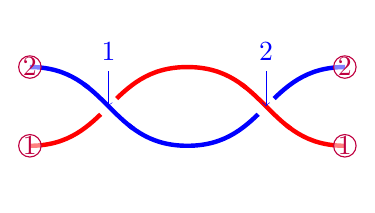
\begin{tikzpicture}
\path (2,1.5) (2,-.5);
\begin{knot}[
draft mode=crossings,
clip width=5,
flip crossing=1,
]
\strand[red,ultra thick] (0,0) .. controls +(1,0) and +(-1,0) ..
(2,1) .. controls +(1,0) and +(-1,0) .. (4,0);
\strand[blue,ultra thick] (0,1) .. controls +(1,0) and +(-1,0) ..
(2,0) .. controls +(1,0) and +(-1,0) .. (4,1);
\end{knot}
\end{tikzpicture} 
  \end{example}
\end{prop}

\begin{definition} {Braid "Multiplication"} { 3 }
  Given braids $\alpha$ and $\beta$, $\alpha \cdot \beta$ is to be obtained by stacking the diagrams of  $\alpha$ and  $\beta.$
  \begin{example} {$\alpha$ and  $\beta$ braids} { 4 }
    \textit {Stack the braids (where bottom nodes of $\alpha$ match up with top nodes of  $\beta$) } \\
    Then, simplify the resulting braid. \\
    This is braid multiplication. \\
  \end{example}
\end{definition}

\begin{definition} {Braid Identity} { 5 }
  The braid that has NO crossings is the identity braid. \\
  Each arc is directly connected to the node below/above it \\
  It has the property that it is the identity under braid multiplication. \\
\end{definition}

\begin{definition} {Braid Inversion} { 6 }
  Given a braid $\alpha$, $\alpha^{-1}$ is to be obtained by reversing the direction of each arc in $\alpha$. \\
  \begin{example} {$\alpha$ braid inversion} { 7 }
    \textit {Every time an arc crossed another in $\alpha$, flip which arc is on top} \\
    This is braid inversion. \\
    \par $\alpha^{-1} \cdot \alpha \equiv I$ \\
  \end{example}
\end{definition}

\begin{example} {$\sigma_i$ braid} { 8 }
  This braid is formed by taking the identity braid and crossing the $i$th and $(i+1)$th strands. \\
  \begin{theorem} {$\sigma_i$ Theorem} { 9 }
    If $\alpha$ is any braid, then  $\alpha$ can always be written as a product of multiple  $\sigma_i$ and  $\sigma_i^{-1}$ braids. \\

  \textit {any braid can therefore be decomposed into a product of $\sigma_i$ and $\sigma_i^{-1}$ braids.} \\
  \begin{note} 
   The decomposition of a given braid is NOT unique. \\
   I.E., multiple different braids can have the same decomposition. \\
  \end{note}
  
 \end{theorem} 
\end{example}

\section {Links}

\begin{definition} {Link} { 10 }
  A \underline{link} is what happens when you take a braid and join the top and bottom dots. \\
  \emph{Links are NOT braids.} \\
  \begin{example} {Link example} { 11 }
    \begin{align*}
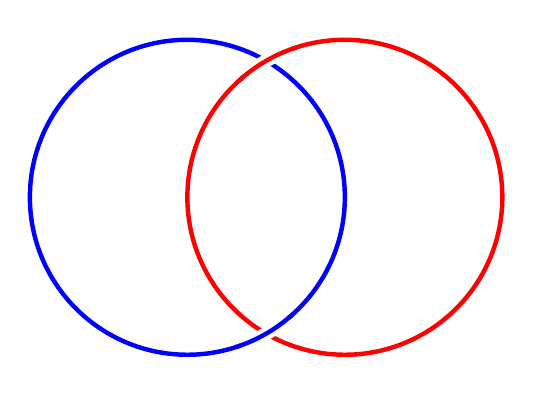
\begin{tikzpicture}
\begin{knot}[
%  draft mode=crossings,
  flip crossing=2
]
\strand (1,0) circle[radius=2cm];
\strand[blue] (-1,0) circle[radius=2cm];
\end{knot}
\end{tikzpicture}
    .\end{align*}
  \end{example}
\end{definition}

\begin{definition} {Trefoil} { 11 }
  A \underline{trefoil} is a link that is a braid of 3 strands. \\
  \begin{example} {Trefoil} { 12 }
    \textit {Draw a braid of 3 strands} \\
    \textit {Join the top and bottom dots} \\
    \textit {This is a trefoil} \\
    \par
    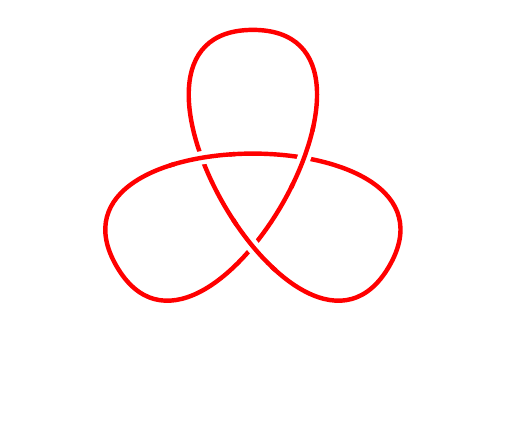
\begin{tikzpicture}
      \begin{knot}[
        consider self intersections=true,
      %  draft mode=crossings,
        flip crossing=2,
        only when rendering/.style={
      %    show curve controls
        }
        ]
      \strand (0,2) .. controls +(2.2,0) and +(120:-2.2) .. (210:2) .. controls +(120:2.2) and +(60:2.2) .. (-30:2) .. controls +(60:-2.2) and +(-2.2,0) .. (0,2);
      \end{knot}
    \end{tikzpicture}
  \end{example}
  
\end{definition}

\begin{prop} {Braid Property} { 13 }
  \underline{Let} $\alpha$,  $\beta$ be braids, then Links of  $\alpha$ and  $\beta$ are identical $ \iff$ you can transform $\alpha$ into  $\beta$ via a sequence of the following moves \\ 
  \par
  This is Markov's Theorem (Not Markov chain Markov!): \\
  \begin{enumerate}
    \item $\gamma \cdot \gamma^{\prime} ~ \gamma^{\prime} \cdot \gamma$
    \item  $\gamma$ 
  \end{enumerate}
\end{prop}
\end{document}
